\documentclass{beamer}
\usepackage{tcolorbox}


\usepackage{tikz}
\usetikzlibrary{arrows,backgrounds,quotes,arrows.meta}
\usepgflibrary{shapes.multipart}

\usepackage{mathtools}
\DeclarePairedDelimiter\ceil{\lceil}{\rceil}
\DeclarePairedDelimiter\floor{\lfloor}{\rfloor}

%\beamerdefaultoverlayspecification{<+->}
\newcommand{\data}{\mathcal{D}}

\DeclareMathOperator*{\argmin}{arg\,min}

\newcommand\Item[1][]{%
	\ifx\relax#1\relax  \item \else \item[#1] \fi
	\abovedisplayskip=0pt\abovedisplayshortskip=0pt~\vspace*{-\baselineskip}}


\usetheme{metropolis}           % Use metropolis theme


\title{Convolutional Neural Networks}
\date{\today}
\author{Nipun Batra}
\institute{IIT Gandhinagar}

\tikzset{
	annotated cuboid/.pic={
		\tikzset{%
			every edge quotes/.append style={midway, auto},
			/cuboid/.cd,
			#1
		}
		\draw [every edge/.append style={pic actions, densely dashed, opacity=.5}, pic actions]
		(0,0,0) coordinate (o-\cubelabel) -- ++(-\cubescale*\cubex,0,0) coordinate (a-\cubelabel) -- ++(0,-\cubescale*\cubey,0) coordinate (b-\cubelabel) edge coordinate [pos=1] (g-\cubelabel) ++(0,0,-\cubescale*\cubez)  -- ++(\cubescale*\cubex,0,0) coordinate (c-\cubelabel) -- cycle
		(o-\cubelabel) -- ++(0,0,-\cubescale*\cubez) coordinate (d-\cubelabel) -- ++(0,-\cubescale*\cubey,0) coordinate (e-\cubelabel) edge (g-\cubelabel) -- (c-\cubelabel) -- cycle
		(o-\cubelabel) -- (a-\cubelabel) -- ++(0,0,-\cubescale*\cubez) coordinate (f-\cubelabel) edge (g-\cubelabel) -- (d-\cubelabel) -- cycle;
		\path [every edge/.append style={pic actions, |-|}]
		(b-\cubelabel) +(0,-5pt) coordinate (b1) edge ["\cubex \cubeunits"'] (b1 -| c-\cubelabel)
		(b-\cubelabel) +(-5pt,0) coordinate (b2) edge ["\cubey \cubeunits"] (b2 |- a-\cubelabel)
		(c-\cubelabel) +(3.5pt,-3.5pt) coordinate (c2) edge ["\cubez \cubeunits"'] ([xshift=3.5pt,yshift=-3.5pt]e-\cubelabel)
		;
	},
	/cuboid/.search also={/tikz},
	/cuboid/.cd,
	width/.store in=\cubex,
	height/.store in=\cubey,
	depth/.store in=\cubez,
	units/.store in=\cubeunits,
	scale/.store in=\cubescale,
	label/.store in=\cubelabel,
	width=10,
	height=10,
	depth=10,
	units=cm,
	scale=.03,
}

\begin{document}
  \maketitle
  
  
  
\section{Computer Vision}

\begin{frame}{Imagenet Challenge}

\end{frame}

\begin{frame}{Some Computer Vision related problems}
Object recognition
Object detection
Style transfer
Visual QA
\end{frame}

\begin{frame}{Fully connected neural networks for images?}
\begin{itemize}
	\item Imagine an image of MNIST size and 1 hidden layer with 100 units, what is \# parameters?
	\item Imagine an image of modern phones (12 Megapixel) and 1 hidden layer with 100 units, what is the \#parameters?
\end{itemize}
\end{frame}

\begin{frame}{Edge Detection}
Apoorv to show vertical and horizontal edge detection on some real image -- write Python code

\end{frame}
%C4W1L02
\begin{frame}{Edge Detection}
Apoorv to show vertical edge detection -- write Python code on a subset of above image say 8 X 8 image (this is made via a seaborn heatmap with annotation ) 
Draw with: https://tex.stackexchange.com/questions/437007/drawing-a-convolution-with-tikz

show multiple images walking through the convlution process
\end{frame}

%C4W1L03
\begin{frame}
Show Sobel, Scharr filter,...
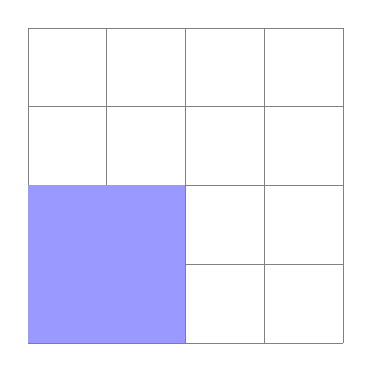
\begin{tikzpicture}
\draw[step=1cm,gray,very thin] (0, 0) grid (4,4);
\fill[blue!40!white] (0,0) rectangle (2,2);


\end{tikzpicture}
\end{frame}

%L04
\begin{frame}
Padding -  makes use of boundary pixels also, the image size does not reduce very quickly

Formula for padding

Valid and Same Convolutions

Padding is generally odd

show animation tikz drawing as done earlier
\end{frame}


\begin{frame}
Strided convolution

Show animation/multiple images as drawn above

show some examples 

\begin{align*}
Size = \floor*{\frac{n+2p-f}{s}+1} \times \floor*{\frac{n+2p-f}{s}+1}
\end{align*}
\end{frame}


\begin{frame}{Convolutions Over Volumnes}
RGB image

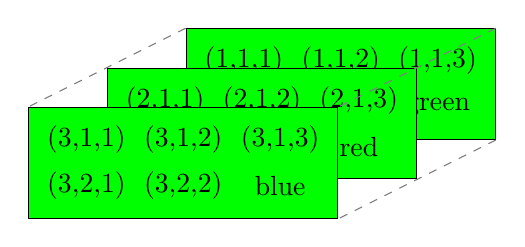
\begin{tikzpicture}
\def\colorPalleteR{green, blue, red}
\def\testarray{{1,-1, 5}}
  \definecolor{myblue}{cmyk}{100,100,255,0}



\def\xs{1} %shift in x direction
\def\ys{0.5} %shift in y direction
\def\nm{3} % number of 2d matrices in the 3d matrix
\foreach \c [count=\x] in {green ,red, blue}
{
	
	\matrix [draw, % for the rectangle border
	fill=green, % so that it is not transparent
	ampersand replacement=\&] %see explanation
	(mm\x)%give the matrix a name
	at(-\x * \xs, -\x * \ys) %shift the matrix
	{
		\node {(\x,1,1)}; \& \node {(\x,1,2)}; \& \node {(\x,1,3)};\\
		\node {(\x,2,1)}; \& \node {(\x,2,2)}; \& \node {\c};\\
	};
}

\draw [dashed,gray](mm1.north west) -- (mm\nm.north west);
\draw [dashed,gray](mm1.north east) -- (mm\nm.north east);
\draw [dashed,gray](mm1.south east) -- (mm\nm.south east);
\end{tikzpicture}
\# channles in image = \# channles in the filter
\end{frame}

\begin{frame}{Multiple Filters}
n . n . nc
\end{frame}

\begin{frame}{One layer CNN}
\end{frame}

\begin{frame}{Summary of notation}
\begin{align}
f^{[l]}: \text{filter size}
\end{align}
\end{frame}

\begin{frame}{Simple CNN example}
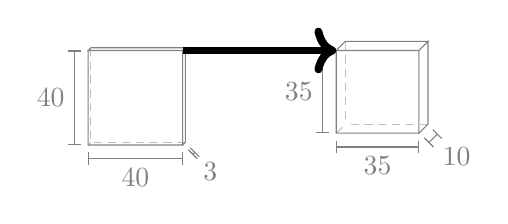
\begin{tikzpicture}

\pic [fill=white, text=gray, draw=gray] at (1,0) {annotated cuboid={width=40, height=40, depth=3,label=A, units=}};

\pic [fill=white, text=gray, draw=gray] at (4,0) {annotated cuboid={width=35, height=35, depth=10,label=B, units=}};

%\pic [fill=white, text=gray, draw=gray] at (6,0) {annotated cuboid={width=15, height=15, depth=20, units=}};

%\pic [fill=white, text=gray, draw=gray] at (8,0) {annotated cuboid={width=5, height=5, depth=40, units=}};


\draw [->, line width=1mm] (o-A) -- (a-B);
\end{tikzpicture}
\end{frame}

\begin{frame}{Types of Layers}
\end{frame}

\begin{frame}{Pooling Layers}
max pooling illustration using images
\end{frame}

\begin{frame}{Why Convolutions work?}
Parameter sharing
Sparsity of connections 
Translation invariant
\end{frame}


\begin{frame}{LeNet-5}
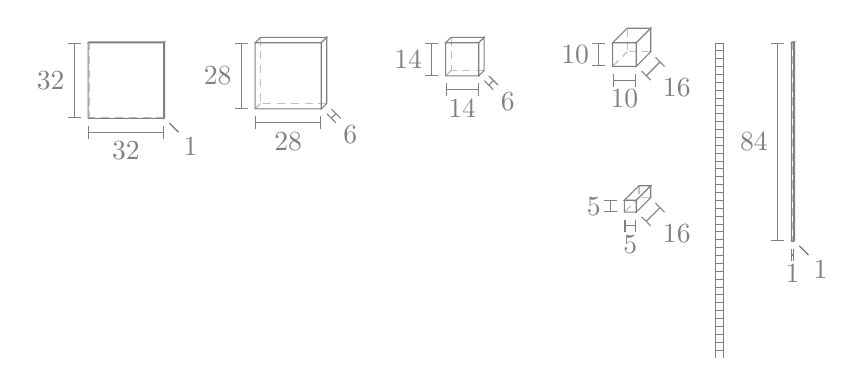
\begin{tikzpicture}

%\pic [fill=gray!20, text=green!50!black, draw=black] at (4,-2) {annotated cuboid={label=A, width=6, height=20, depth=15, units=mm}};

%\pic [fill=red!20, text=green!50!black, draw=black] at (4,-2.7) {annotated cuboid={label=B, width=2, height=4, depth=3, units=m, line=dashed}};

%\pic [fill=blue!20, text=green!50!black, draw=black] at (5,-2) {annotated cuboid={label=C, width=6, height=20, depth=15, units=mm}};

%\pic [fill=green!20, text=green!50!black, draw=black] at (4.8,-2.7) {annotated cuboid={label=D, width=2, height=2, depth=2, units=m, line=dashed}};

%\pic [fill=orange!20, text=green!50!black, draw=black] at (5.5,-2.3) {annotated cuboid={label=E, width=3, height=10, depth=7, units=m, backline=draw}};

%\draw (e-B) -- (a-D);
\pic  [fill=white, text=gray, draw=gray] at (0,0) {annotated cuboid={width=32, height=32, depth=1,label=A, units=}};

\pic [fill=white, text=gray, draw=gray] at (2,0) {annotated cuboid={width=28, height=28, depth=6, label=B, units=}};

\pic [fill=white, text=gray, draw=gray] at (4,0) {annotated cuboid={width=14, height=14, depth=6,label=C, units=}};

\pic [fill=white, text=gray, draw=gray] at (6,0) {annotated cuboid={width=10, height=10, depth=16, label=D, units=}};

\pic [fill=white, text=gray, draw=gray] at (6,-2) {annotated cuboid={width=5, label=E, height=5, depth=16, units=}};

%\pic [fill=white, text=gray, draw=gray] at (7,0) {annotated cuboid={width=1, height=120, label=F, depth=1, units=}};

\pic [fill=white, text=gray, draw=gray] at (8,0) {annotated cuboid={width=1, height=84, depth=1, label=G, units=}};
%\pic [fill=gray!20, text=green!50!black, draw=black] at (4,-2) {annotated cuboid={label=A, width=6, height=20, depth=15, units=mm}};
%\node[text width=3cm] at (10, -1) ;
%\draw (A) -- (B);

\draw[step=0.1cm,gray,very thin] (7, 0) grid (7.12, -4);


\end{tikzpicture}
\end{frame}

\begin{frame}{AlexNet}
\end{frame}

\begin{frame}{VGG}
\end{frame}




\end{document}